\chapter{Experiments}
\label{ch:experiments}
In the \autoref{sec:building model} is described how the grey-box model of the building is created. However, it is not nearly explained where the data comes from. Experiments have been conducted specifically to obtain this data. These experiments are explained in this separate chapter. \newline
This thesis is developed during the summer, thus no data from the reference building with a non-zero control signal $\dot{Q}_\text{heating}$ are available. To acquire data with the varying control signal, we heat the reference building with electric heaters in two experiments, one for verification data and one for training data. Therefore, the sensors of the building record the temperature curves in the rooms and the electrical consumption of the building. The experiments are under the assumption that the whole electrical power of the heaters and other consumers of power, such as lights and office devices, is changed in heat.

\section{Experiment 1}
\label{sec:Experiment1}

\subsection{Background to the experiment 1}
\label{subsec:Backgroud to experiment 1}
The feasibility of the first experiment on the reference building is unclear. To be able to simply repeat the experiment in the event of an error, the experiment with the smaller data set is conducted at first. Hence, the first experiment aims to obtain the data for the verification period, which is shorter than the training period. Furthermore, the experiment is conducted over a weekend (from 16. July to 18. July 2021), as we reduce interference from occupants, such as opening doors or windows, and we enable the occupants a comfortable working temperature. Therefore, all windows and doors are opened after the experiment to cool down the building. At last, there should be no electrical charging of the cars during the experiment, because this electricity consumption has the same measuring point as the electricity consumption of the entire building. This would disrupt the assumption that all electrical power is converted into heat.\newline
At first, we set up the household heater without a fan in room 1, the household heater with a fan in room 2, and the industrial heater in floor 2 (see \autoref{fig:Bauplan}). The heaters are selected based on availability so that no new equipment has to be purchased. Some technical information and the configuration of the heaters are described in \autoref{tab:HeatersData}.
\begin{table}[]
    \centering
    \begin{tabular}{p{3.1cm}|c|p{5.3cm}|p{5.7cm}}
    Heater & Acronym & Technical data & Configuration \\
    \hline
     Household Heater without a Fan & HoHe &
     \begin{itemize}
     \item maximum power: $2000 W$
     \item closed-loop control
     \end{itemize}
     & \begin{itemize}
     \item switch symbol: $|$
     \item temperature setting: $5 - 6$
     \end{itemize}  \\
     Household Heater with a Fan & HoHeF &\begin{itemize}
     \item maximum power: $2000 W$
     \item open-loop control
     \end{itemize}
     & \begin{itemize}
     \item switch symbol: $750 W$
     \end{itemize}  \\
     Industrial Heater & IH &
     \begin{itemize}
     \item maximum power: $9000 W$
     \item closed-loop control
     \end{itemize}
     & \begin{itemize}
     \item switch symbol: 
\begin{tikzpicture} [thick, scale=0.3]
    \fill [black] (0,0) rectangle (1.5cm,0.7cm) ;
    \end{tikzpicture}
     \item temperature setting: middle
     \end{itemize}  \\
    \end{tabular}
    \caption{Technical data and configuration during the experiments}
    \label{tab:HeatersData}
\end{table}
\nomenclature[A]{HoHe}{Household Heater without a fan}
\nomenclature[A]{IH}{Indusrial Heater} 
\nomenclature[A]{HoHeF}{Household Heater with a Fan}

\subsection{Data of the experiment 1}
\label{subsec:Data of the experiment 1}
A more exact sequence of the experiment is showing in \autoref{tab:Experiment1app} as laboratory journal or in the \autoref{fig:P_elTemperatureExperiment1} with the data. The Figure presents the electrical consumption $P_el$ and the air temperatures in rooms 1 and 2, the kitchen, and floor 2 of the reference building from the beginning to the ending of the experiment. The start is marked by switching on the heaters in floor 2 and rooms 1 and 2. In the end, the heaters are switched off in room 1, the kitchen and floor 2. \newline 
The data demonstrate the behaviour of the heaters. Consequently, in floor 2, the IH switches often on and off due to the closed-loop control. Therefore, IH generates the fluctuations in the increasing air temperature curve. At the same time, we notice the on and off of the heater in $P_el$ at the high peaks. The HoHe has the same behaviour as the IH but with a smaller influence on the air temperature in room 1 due to its lower power. \newline
Only the HoHeF is controlled open-loop and heats constantly with $750 W$ the room air, where we remark no fluctuations in the temperature rise. Because the HoHeF does not switch off independently and we have sunny days during the experiment, some temperatures, e.g. the screed temperature, are nearly below 40°C. To avoid a too-hot room for the occupants after the experiment, we stop heating room 2 on Saturday night and rearrange the HoHeF in the kitchen. Since we average the temperature in all rooms for the model estimation from \autoref{ch:modelling}, it is not relevant which room is heated.
\begin{figure}
            \centering
            %\def\svgwidth{100pt}
            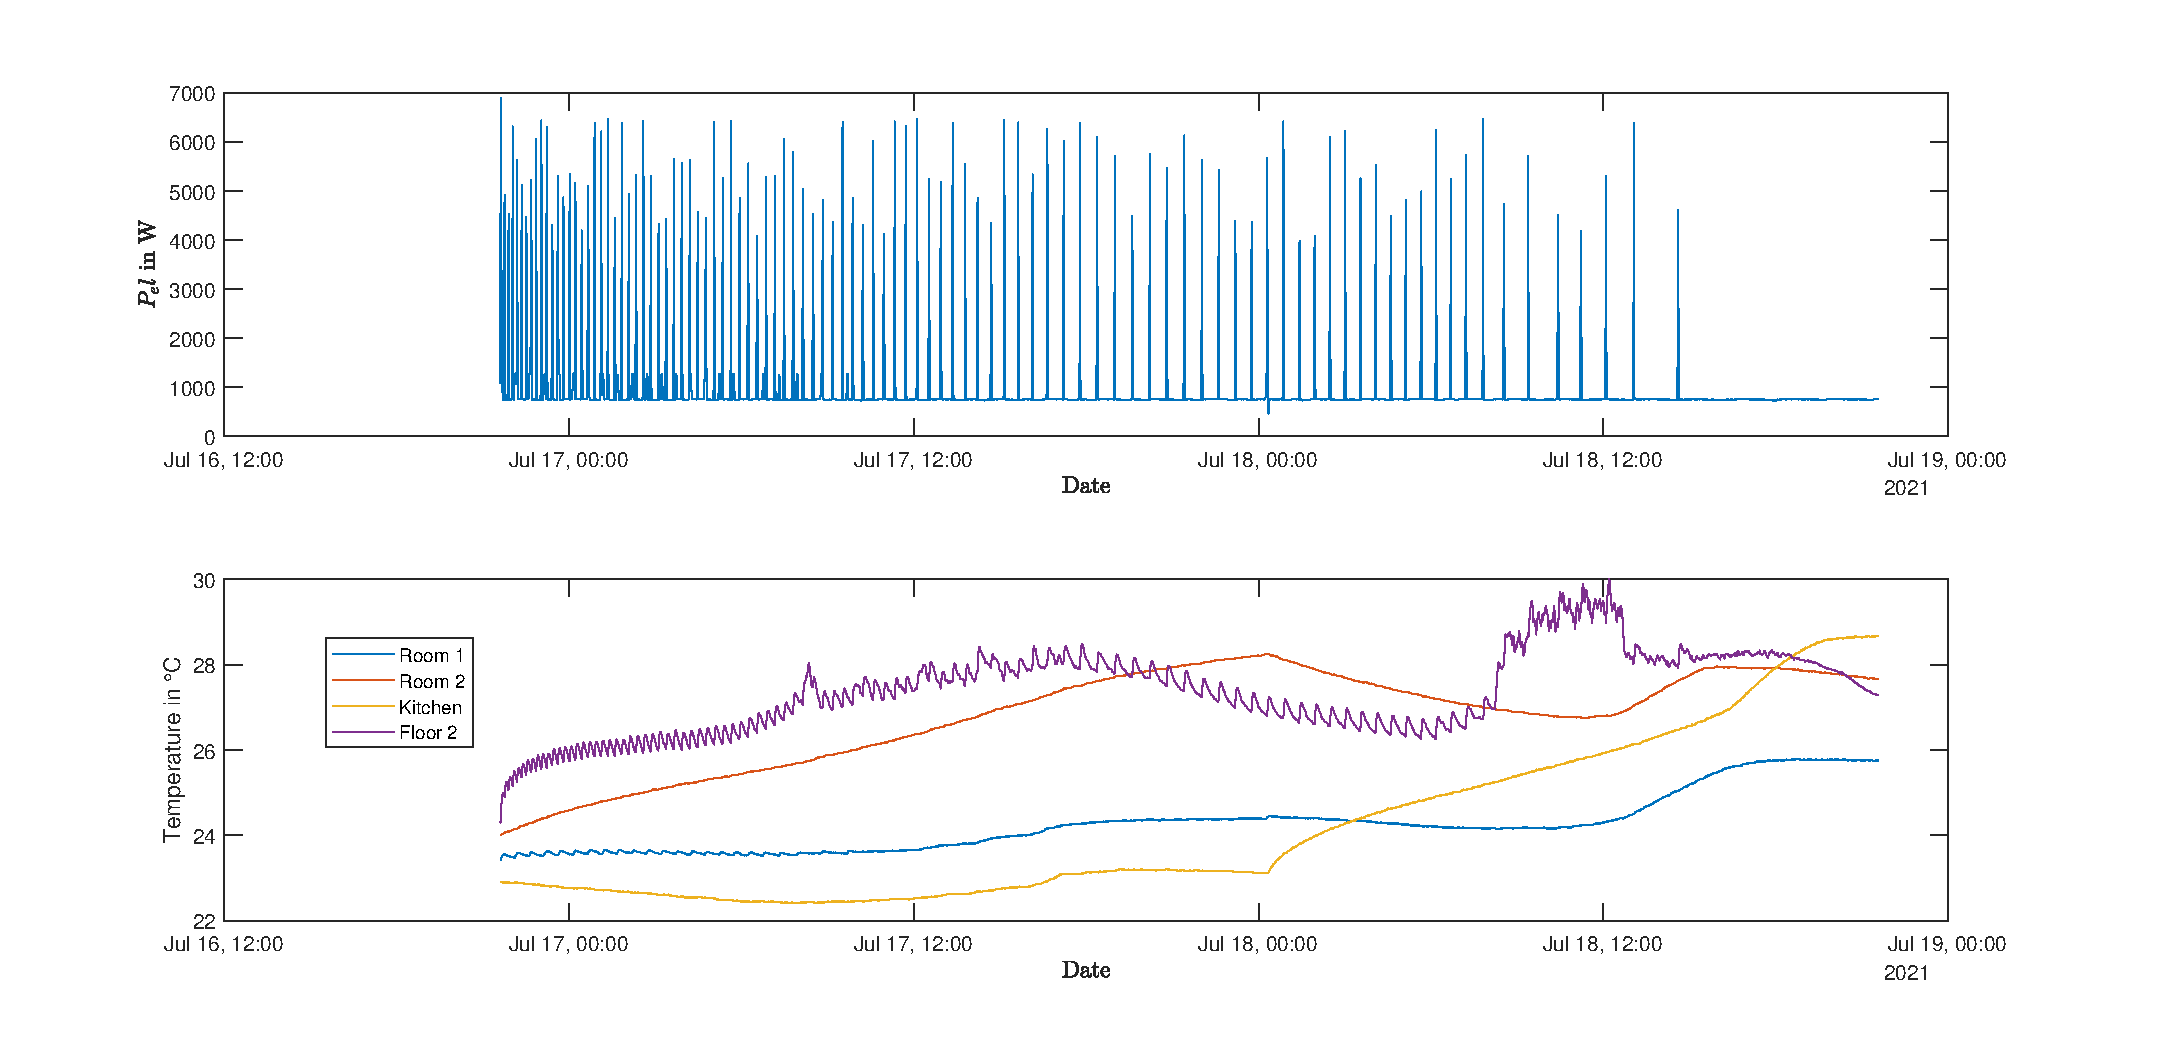
\includegraphics[width=0.85\textwidth]{figure/P_el_trainingsdaten_latex.eps}
           \caption{Electrical consumption of the building and air temperature inside the rooms during the experiment 1}
           \label{fig:P_elTemperatureExperiment1}
    \end{figure}
\section{Experiment 2}
\label{sec:Experiment2}
Programmable logic controller (PLC)

\subsection{Background to the experiment 2}
\label{subsec:Backgroud to experiment 2}

\subsection{Data of the experiment 2}
\label{subsec:Data of the experiment 2}
\begin{figure}
            \centering
            %\def\svgwidth{100pt}
            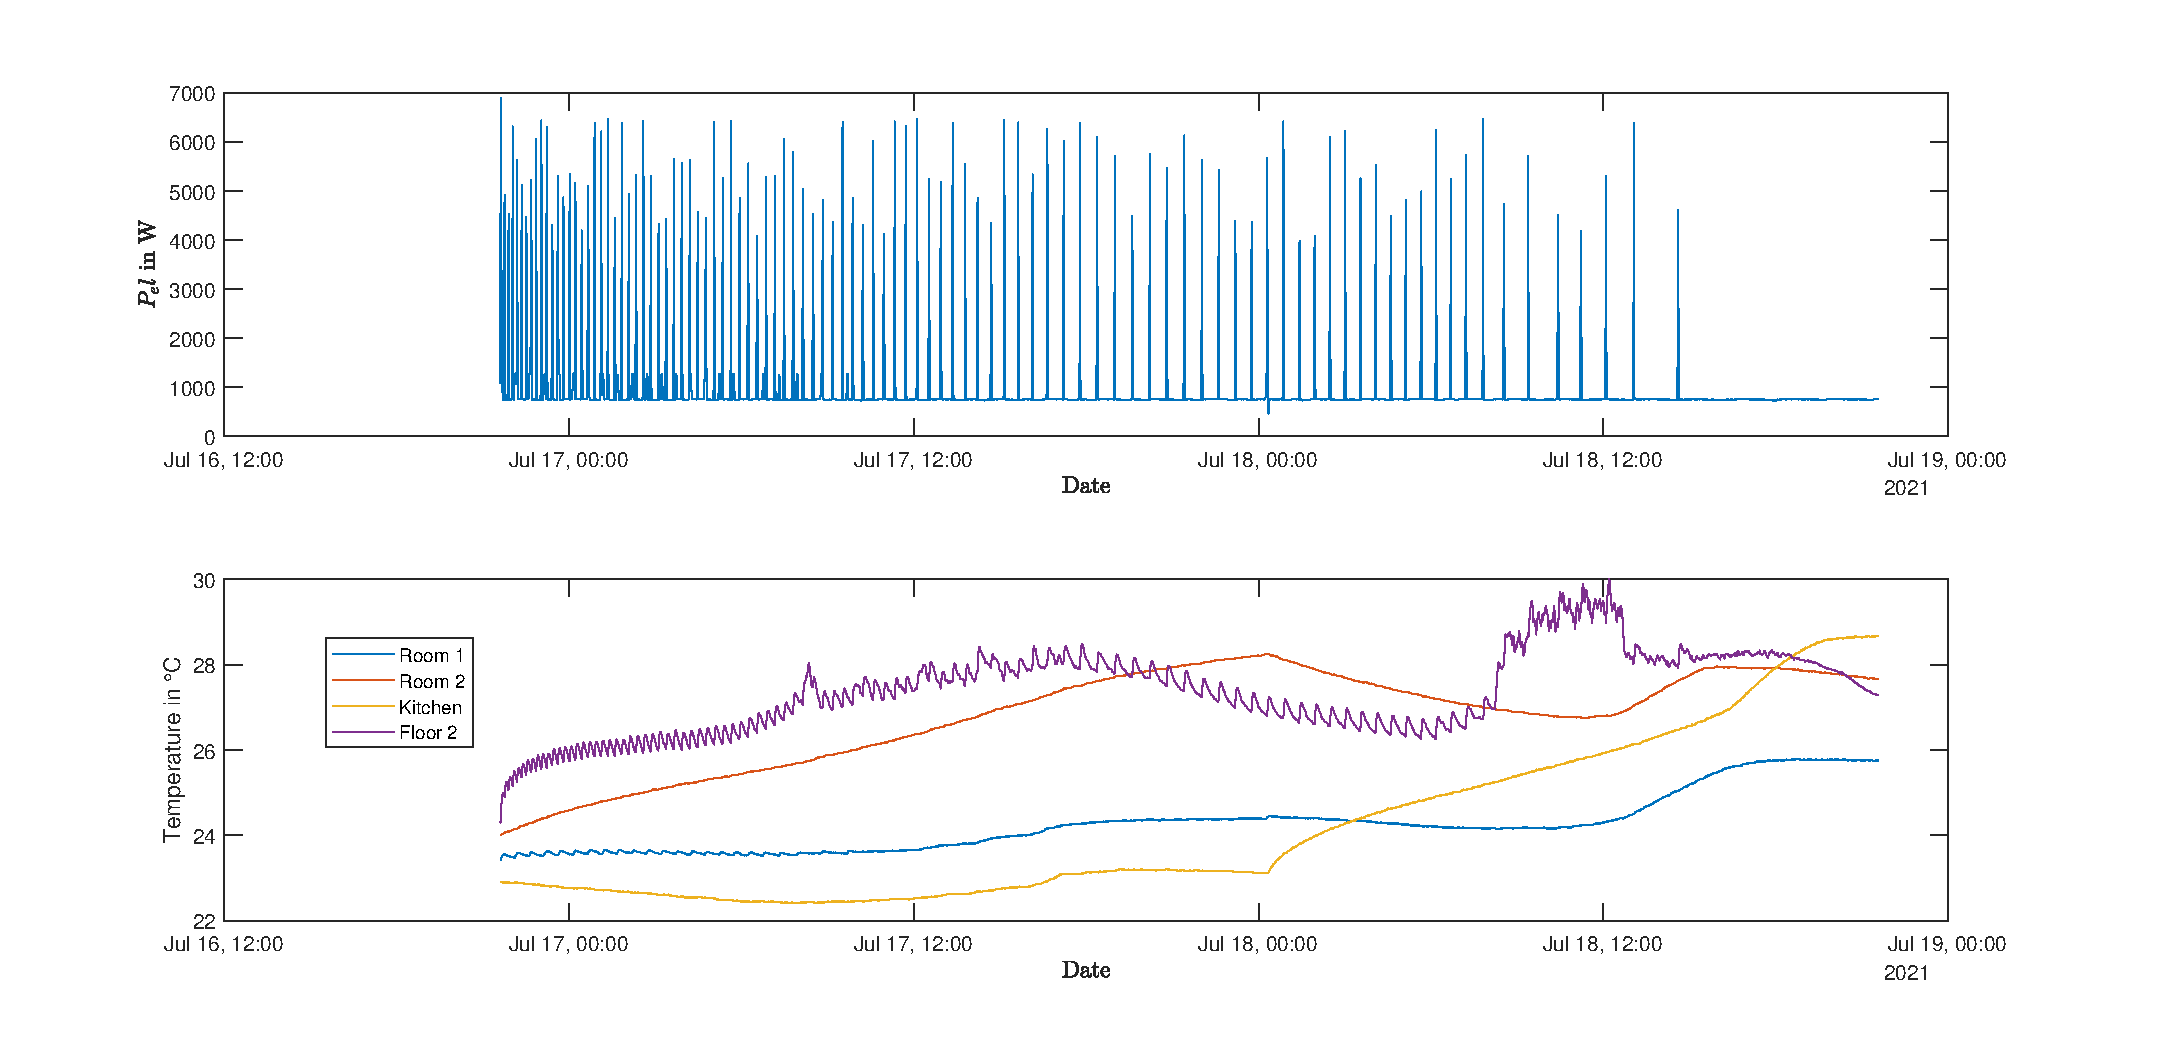
\includegraphics[width=0.85\textwidth]{figure/P_el_trainingsdaten_latex.eps}
           \caption{Electrical consumption of the building and air temperature inside the rooms during the experiment 1}
           \label{fig:P_elTemperatureExperiment1}
    \end{figure}
\section{Findings of the experiments}
\label{sec:findings of the experiments}
